\documentclass{article}
\author{
  Torrent Gorjon, Xavier\\
  \texttt{Xavier.TorrentGorjon@os3.nl}
}
\title{Protecting against relay attacks forging increased distance reports}

\usepackage{graphicx}

\usepackage[backend=bibtex]{biblatex}

\bibliography{references}


\begin{document}


\begin{titlepage}
\center
\textsc{}\\[1cm]
\textsc{\LARGE Universiteit van Amsterdam}\\[1.5cm]

\textsc{\Large Research Project I}\\[0.5cm]

\textsc{\Huge Protecting against relay\\[0cm] attacks forging increased\\[0.5cm] distance reports}\\[1.5cm]


\includegraphics[scale=1]{images/uva.png}\\[1cm]

\begin{minipage}{0.5 \textwidth}
\begin{center} \large
Xavier Torrent Gorj\'{o}n\\
\emph{Xavier.TorrentGorjon@os3.nl}\\[0.5cm]
\end{center}
\end{minipage}\\[2cm]
{\large \today} 


\end{titlepage}


\newpage


\renewcommand{\abstractname}{\Large Abstract}
\begin{abstract}
Lorem ipsum dolor sit amet, consectetur adipiscing elit. Sed sed diam metus. Quisque velit urna, dictum vel eros eu, congue luctus augue. Nulla sit amet metus nec ipsum pretium vestibulum ut quis sem. Nullam malesuada risus ut rhoncus consequat. Fusce in hendrerit nibh. Morbi a magna nunc. In vel justo tincidunt, porttitor tellus in, porta lacus. Nulla posuere enim arcu, eget aliquet mauris dictum ornare. Morbi iaculis nec elit vitae rutrum. Nam posuere, risus sed semper finibus, augue lorem blandit ex, non tempor nunc tortor vel arcu. Cras non tortor ipsum. Suspendisse vestibulum molestie nibh, lacinia efficitur nunc luctus non. Phasellus sed nibh at est suscipit pulvinar. Cras eleifend ante et volutpat suscipit.
\end{abstract}

\newpage





\tableofcontents





\newpage





\section{Introduction}
\label{sec:introduction}

Communications between machines face many challenges when the transmitted information needs to be protected. Most communications can prove to be valuable attack points for third parties that want to recover, modify, block or otherwise manipulate the original message sent for personal profit. Part of these attacks can be prevented by using end to end encryption and signature of the data. However relay attacks cannot be prevented just by using cryptographic algorithms.

Relay attacks consist on the mere reception and replay of information. Although at first this might seem harmless, many systems become vulnerable if that relaying of information is not noticed. One scenario that can be used as an example of the threat these attacks represent are access control systems, in which a device is used to prove that a user is within a certain distance from a validator through a challenge-response protocol. On unprotected implementations of these access control systems, an attacker can relay the challenge from the validator to a valid user who is not in range and relay its answer back to the validator, effectively bypassing distance validation. Practical attacks on this kind of systems have been demonstrated on various studies, as in \cite{francillon2011relay, francis2010practical, hancke2005practical, markantonakis2012practical}.

In this paper, we will first discuss the relay attacks used to forge fake location positions, focusing on the countermeasures against them. We will then focus on attacks forging increased distance reports, the feasibility of these attacks and propose solutions to them. In Section \ref{sec:relatedwork} we will discuss the available literature on this topic. In Section \ref{sec:background} we will briefly present results and conclusions from our research in the available literature about distance bounding protocols, GPS, radar detection and Inertial Navigation System. We will present on Section \ref{sec:researchquestions} a more detailed explanation on the research questions this project aims to answer. Following on Section \ref{sec:methodology} we will explain the methodology used in this study. Section \ref{sec:results} will discuss the actual results from our research questions, after which we will provide conclusions about the results gathered in Section \ref{sec:conclusions}.







\section{Related Work}
\label{sec:relatedwork}

Relay attacks have been for long, and continue to be, an extensive field of research, as technologies and devices are shifting to a more mobile-focused paradigm. Many old procedures are being enhanced with wireless features, such as credit cards and car keys. However, it is not possible to find in the available literature studies regarding relay attacks used to fake increased distances between two legitimate nodes. It is the goal of this project to prove that these attacks can prove to be a real threat in real world applications, and how current distance bounding protocols can be enhanced to limit their vulnerability against them.

There is much literature available presenting solutions to distance bounding problems, as \cite{brands1994distance, tu2007rfid, rasmussen2010realization}. All of these studies are used as a base for others in a constant iteration to improve the protocols. As new attacks emerge against distance bounding protocols, new studies are published to fix the deficiencies of the previous work. This project will use part of these studies as a basis for the solutions against the studied relay attacks.

There are also many practical studies in the field of distance bounding, which aim to test the vulnerabilities on real applications, such as \cite{francillon2011relay, francis2010practical, hancke2005practical, markantonakis2012practical, vandenbreekel2014relay}. Although all that research refers to forging decreased distance reports and it is not directly used in our research, it has been deeply as an starting point and inspiration.

This project will assume certain conditions for the studied attacks. Some assumptions and justifications will be required on the investigation, based on the characteristics of GPS signals. Many studies focus on the feasibility of intentional attacks against GPS systems, as \cite{warner2003gps, wen2005countermeasures, jafarnia2012gps}. These studies conclude that, even though spoofing is hard with the solutions they propose, it is not impossible. With this premise, the goal will be to develop countermeasures against relay attacks without relying on GPS signals.

In a similar way to GPS signals, other systems such as Radar location \cite{cadirci2009rf} and Inertial Navigation Systems \cite{patent:4085440} could be arguably used to prevent this attacks. Using these information sources we will explain why these systems are not reliable neither, reaffirming the need of a modified distance bounding protocol that is not vulnerable to relay attacks.

Finally, this study is closely related to the field of MANETs (Mobile Ad-hoc NETworks), and as such, literature available in this topic is of our interest. In particular, wormhole attacks (\cite{hu2006wormhole, maheshwari2007detecting, goyal2010literature}) are a specific type of relay attack that, while being different than the ones we will study in this document, provide insight to our investigation as they are closely related.








\section{Background}
\label{sec:background}

In this section we will discuss distance bounding protocols, the GPS system and radar detection. All of them are extremely relevant topics to our research. First we will explain the current distance bounding protocols, as we will use them as a starting point for our research. Then we will move onto GPS, and explain why systems shouldn't rely completely on it, hence the need to develop more powerful distance bounding protocols for our study cases. Lastly, we will discuss the possibility of using radar detection and Inertial Navigation System to fight the proposed attack.

\subsection{Distance bounding}

Distance bounding protocols were developed as a response to relay attacks that attempt to fool systems that validate an users proximity to a validation point. Common scenarios of these applications are found in access control systems, such as smartcards to access buildings or cars using remote passive keys.

These attacks try to use properties of the systems used in the communications (such as signal intensity or message time of flight (ToF)) to validate the proximity of users. Based on the work of \citeauthor{capkun2006secure} in \cite{capkun2006secure}, we will proceed to briefly discuss these methods:

\begin{description}
  \item[Signal Intensity] Signal intensity protocols try to achieve proper location of other nodes by measuring the received signal strength. Previous work available in the public literature, such as the research by \citeauthor{seshadri2005bayesian} in \cite{seshadri2005bayesian} proves the usefulness of this location system. Even though attacks on this systems are hard to perform \cite{sheng2008detecting}, the defences against them rely mostly on anomaly detection. The reliability of these systems can be decreased in heavily adverse situations, and the ToF methods discussed next provide a higher degree of security.
  \item[Ultrasound ToF] Ultrasound ToF measures the round-trip time of messages sent and received from the parties measuring the distance between them. This does not depend on the signal strength for the measurement, although ultrasound-based ToF has the latent vulnerability that other methods such as radio frequency or optical wires attackers can surpass the speed of the ultrasound communication, effectively being able to relay information faster than the legitimate infrastructure.
  \item[Radio ToF] Radio-based ToF uses the same method as ultrasound ToF to perform the distance check. The key of the success of this method is that the information transmitted travels at speeds near the speed of light, meaning there is no physical way to fake one node is closer than it really is. Practical studies on this method \cite{rasmussen2010realization} developed hardware that can perform the operations required under 1ns, meaning that the maximum theoretical distance an attacker can shorten its reported distance is under 15cm.
\end{description}

In this project we will be using Radio ToF as a basis for our work, as it is proven to be the most secure and reliable method. However, this method alone is not enough to fight reports that forge an increase on the real distance between parties, and this will be the main focus of our research.

\subsection{GPS location}

It could be argued that GPS location can be used to prevent the attacks that we will discuss on the next Section. However, GPS signals have their own weaknesses both with and without presence of adversaries.

In settings without adversaries, GPS positioning cannot be reliably used indoors or underground, and sometimes the presence of tall buildings or structures nearby is enough to disrupt its data.

Speaking of scenarios with one or multiple adversaries, even though there are many countermeasures to prevent attacks against GPS positioning \cite{warner2003gps, wen2005countermeasures, jafarnia2012gps}, there do not provide complete security, similar to the Signal Intensity location protocol.

Due these problems, he U.S. government actually recommends to always have backup systems for GPS and suggests to never rely entirely on it\footnote{\url{http://www.gps.gov/support/faq/#jamming}}. Based on these premises we will assume that GPS is not a part of our system, or that we cannot rely on it.

\subsection{Radar detection}

One way to protect against this kind of Man-In-The-Middle attack could be by attempting to physically detect the attacker. If an unidentified object is detected between the parties and it is confirmed that it does not belong to the system, security measures could be taken to prevent such relay attacks.

However, recent studies as the one by \citeauthor{cadirci2009rf} in \cite{cadirci2009rf}, state that Radar Cross Section,a measurement used to rate the ability to reflect radar waves by an object, can be heavily decreased by employing proper techniques such as the usage of special materials, radiowave-absorbing paint and specific shapes that minimize and disperse radio reflection.

As a real world example, the first operational aircraft designed to employ advanced stealth technology, the Lockheed F-117 Nighthawk from the United States Air Force, with a wingspan and a length of $13.20m$ and $20m$ respectively\footnote{\url{http://www.fighter-planes.com/info/f117_nighthawk.htm}}, has a RCS signature of $0.025m^2$, which is similar to that of a bird\cite{cadirci2009rf}.

In the attack scenarios proposed on Section \ref{sec:results}, flying drones would be the most versatile device to perform the attacks. Considering these drones can be considerably smaller than these aircraft (depending on the situation, the used drone could be shorter than $1m$ in length, height and width), it is easy to foresee that they would be almost invisible to radar systems. If the attack scenario does not require the attacker to fly at relative high speeds, its RCS signature could be further decreased by designing an attack drone with a shape specifically made to absorb radar waves. 

We therefore conclude that, in the current state of stealth and anti-stealth technologies, radar detection would not be a strong countermeasure to prevent against that kind of attacks.



\subsection{Inertial Navigation System}

Inertial Navigation Systems are devices used to provide machines a sense of self-awareness of their current position, based on their initial position and the chosen routes, by using accelerometers and gyroscopes. These systems could be relevant for this research, as they share the same \emph{relative positioning} focus, staying independent from third party sensors.

The work done by \citeauthor{woodman2007introduction} in \cite{woodman2007introduction} evaluates the cost and performance of the INS. The conclusion from that work is that available INS hardware cannot realistically provide an accuracy below $5m$ of error after $60$ seconds of operation. In an environment with multiple nodes using this system, this means that after $60$ seconds, the location detection between two nodes could be as biased as $10m$. This also limits is usability as a stand-alone positioning system, as the error will only grow larger as time goes on.

Although INS accuracy is rapidly improving over the years, right now is not a viable solution or countermeasure to our problem.







\section{Research Questions}
\label{sec:researchquestions}

As seen in the Related Work section, on the current literature there are no proposals to fight the subset of relay attacks that attempt to fake increased distance reports between legitimate parties. This project will prove that these attacks suppose a real threat, and as such, our first research question will be:\\

\emph{How feasible are forged increased distance report relay attacks?}\\

Additionally, after the demonstration of the possibilities of these attacks, a second research question is considered:\\

\emph{How can these attacks be prevented?}

\subsection{Feasibility of forged increased distance report relay attacks}

Minimum distance bounding appeared to have many solutions on the current literature. However, we observed that distance bounding regarding upper limits on reported distances was not a subject of research. In this project, we will present some theoretical attacks that could be used on many real world scenarios, and propose variations on the current distance bounding protocols to solve them.

The proposed scenarios are diverse in both context and properties of the systems involved in the communications. We will focus the study from the point of view of systems involving communication between drones, although we will provide solutions that can be extrapolated to other systems as well, such as automatically driven cars.

In this research question, we ultimately aim to explain why these attacks can be dangerous and an interesting topic of research.

\subsection{Preventing forged increased distance reports}

The second research question will focus on providing solutions to the issues stated on the first. Unlike minimum distance bounding protocols, we won't be able to use the speed of light as a fact to develop responses that cannot be faked, which implies that we might not be able to develop a system that completely protects against these increased distance reports. However, we do expect to provide solutions that suppose a meaningful security increase against these attacks.









\section{Methodology}
\label{sec:methodology}

As stated in the Introduction and the Related Work sections, there are reasons to see relay attacks that fake increased distance reports as a threat.

Using the information gathered and stated in the Background section, we will first study the conditions under which distance bounding systems could be vulnerable to these attacks. We will present many real life applications of distance bounding protocols whose intended functionality could be altered by performing these attacks.

Afterwards, using the mentioned sources of information, variations to the distance bounding protocols will be proposed, in order to effectively reduce the threat these attacks suppose.

Using a theoretical approach, an explanation and evaluation of both the feasibility of these attacks as well as the proposed solutions will be given.











\section{Results}
\label{sec:results}

On this section we will present the results of our research, structured in the form of two research questions.

\subsection{Feasibility of forged increased distance report attacks}

The theoretical attack we propose relies on the fact that the discussed protocols regarding distance bounding on the available literature do not prevent relay attacks that report an increased distance between two legitimate parties.

The basics of the attack are easy to understand. Assume two parties are communicating using a transmitter-receiver model, that is, one of them is actively reporting its position to the other. At some point, an attacker seizes a position between them and starts disrupting the communication between them, either by attempting to block the communication or by jamming its frequency range. At the same time, he starts recording the information and resending it to the receiver node, adding a brief delay on it. Figure \ref{fig:attackexample1} provides a graphical description of the problem. The effectiveness of this attack can be increased by having multiple malicious nodes attempting to block the original signal.

\begin{figure}[h!]
  \centering
    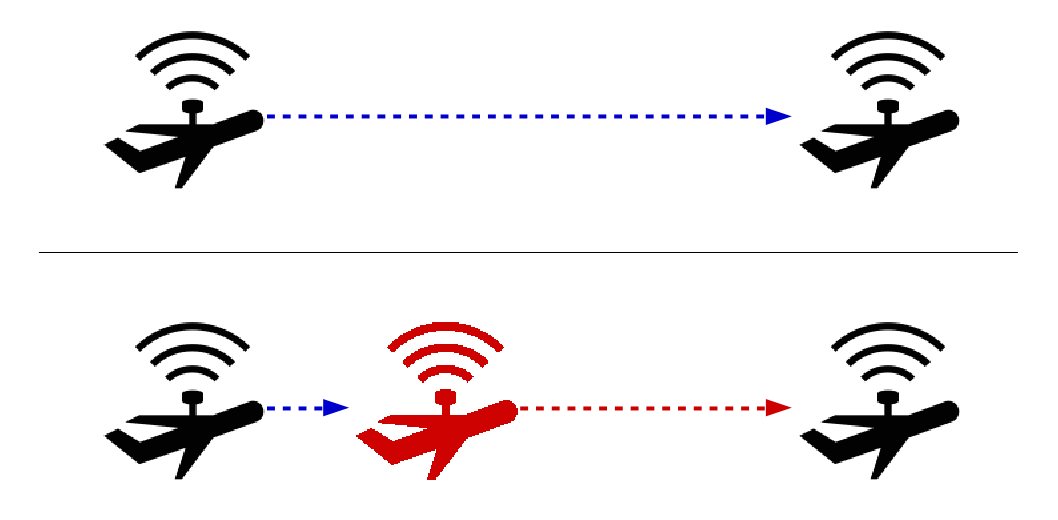
\includegraphics[width=0.8\textwidth]{images/attack1.png}
  \caption{Regular communication versus block and relay attack.}
  \label{fig:attackexample1}
\end{figure}

Many systems use these distance reporting protocols for their pathing decisions. This kind of attack could cause unexpected behaviour on the systems, effectively altering their original desired outcome. 

Such attacks are difficult to perform in practice, as they require relaying and jamming communications at the same time. Appropriate timing on the relay and some degree of knowledge about the system are also required to successfully perform an attack. However, there is no proving that these attacks cannot be performed with the appropriate technology.

Following next

\subsubsection{Autonomous cars}
Present diverse attack scenarios. [at least 1 paragraph per case]
   Drones (multiple cases)
     Cooperative working
     Area surveillance
   Automatically driven cars
   Boats and harbours
  ...?
For each case, state clearly the assumptions made and its limitations


\subsection{Fighting forged increased distance reports}

Present the solutions

Multiple antenas and shared knowledge [Various paragraphs (5+), this is the first solution]










\section{Conclusions}
\label{sec:conclusions}

Consider the theoretical assumptions of the project [1 paragraph]

Given the proposed solutions, introduce and explain the implications [2 or more paragraphs]










\section{Future Work}
\label{sec:futurework}

Briefly talk about the need of a more practical study with real hardware [1 paragraph]

...?











\section{Acknowledgements}
\label{sec:acknowledgements}

[2 paragraphs max]

\printbibliography


%%% APPENDIX

\end{document}
